\documentclass[conference]{IEEEtran}
\usepackage[T1]{fontenc}
\usepackage[utf8]{inputenc}
\usepackage{graphicx}
\usepackage{booktabs}
\usepackage{amsmath}
\usepackage{amssymb}
\usepackage{tikz}
\usetikzlibrary{arrows.meta, positioning, shapes.geometric, fit, backgrounds, calc}
\usepackage[colorlinks=true,linkcolor=blue,citecolor=blue,urlcolor=blue]{hyperref}

% ------------------------------------------------------------------
% Headline macros: % PLACEHOLDER -- overwritten by prototype/experiments/make_tables.py
% (interim compile stub; Task 7 greps for this marker before submission)
\newcommand{\SPVanilla}{0.000}
\newcommand{\SPRAG}{0.000}
\newcommand{\SPCoVe}{0.000}
\newcommand{\SPHealGen}{0.000}
\newcommand{\SPGoldVanilla}{0.000}
\newcommand{\SPGoldRAG}{0.000}
\newcommand{\SPGoldCoVe}{0.000}
\newcommand{\SPGoldHealGen}{0.000}
\newcommand{\SPMicroHealGen}{0.000}
\newcommand{\HRHealGen}{0.000}
\newcommand{\AnyHRHealGen}{0.000}
\newcommand{\EMHealGen}{0.000}
\newcommand{\EMRAG}{0.000}
\newcommand{\FscoreHealGen}{0.000}
\newcommand{\RetrHealGen}{0.0}
\newcommand{\LatHealGen}{0.0}
\newcommand{\ECEHealGen}{0.000}
\newcommand{\NAbl}{150}
\newcommand{\NTest}{150}
 is GENERATED by
% prototype/experiments/make_tables.py from results/*.csv.
% Never hand-edit values there; never type measured numbers inline.
% ------------------------------------------------------------------

\title{HealGen: Claim-Level Evidence-Sufficiency-Guided Self-Healing
Inference for Factual LLM Generation}

% Byline intentionally deferred to Phase D (design spec §8.2: solo vs.
% faculty-supervisor byline decided at submission).
\author{ PLACEHOLDER-BYLINE
\thanks{Draft manuscript -- HealGen prototype results, generated from
committed experiment outputs.}}

\begin{document}

% Headline macros are input OUTSIDE the abstract environment: IEEEtran's
% abstract creates a TeX group, which would scope \newcommand away.
\IfFileExists{tables/headline.tex}{% PLACEHOLDER -- overwritten by prototype/experiments/make_tables.py
% (interim compile stub; Task 7 greps for this marker before submission)
\newcommand{\SPVanilla}{0.000}
\newcommand{\SPRAG}{0.000}
\newcommand{\SPCoVe}{0.000}
\newcommand{\SPHealGen}{0.000}
\newcommand{\SPGoldVanilla}{0.000}
\newcommand{\SPGoldRAG}{0.000}
\newcommand{\SPGoldCoVe}{0.000}
\newcommand{\SPGoldHealGen}{0.000}
\newcommand{\SPMicroHealGen}{0.000}
\newcommand{\HRHealGen}{0.000}
\newcommand{\AnyHRHealGen}{0.000}
\newcommand{\EMHealGen}{0.000}
\newcommand{\EMRAG}{0.000}
\newcommand{\FscoreHealGen}{0.000}
\newcommand{\RetrHealGen}{0.0}
\newcommand{\LatHealGen}{0.0}
\newcommand{\ECEHealGen}{0.000}
\newcommand{\NAbl}{150}
\newcommand{\NTest}{150}
}{}

\maketitle

\begin{abstract}
% Numbers only via generated macros (\S tables/headline.tex); the
% \IfFileExists guard lets interim compiles run before results exist.
Large language models hallucinate factual claims, and existing remedies
either retrieve for every question or verify only after the fact.  We
present HealGen, a draft-first self-healing architecture that decides,
per atomic claim, whether to trust it, retrieve evidence for it, or
repair it locally: a claim-level risk estimator, an evidence-sufficiency
predictor gating retrieval, a dynamic claim--evidence graph, and
localized repair, all driven by one validated NLI judge.  We pair the
architecture with an evaluation protocol designed to make such claims
checkable: the judge scores every system against one frozen shared pool
per question (gold knowledge plus the union of all four systems'
passages, so no system's retrievals are private evidence; a gold-only
condition is also reported), itself passes a pre-registered validation
gate before any benchmark run, and scores the \emph{emitted} answer
rather than private intermediate
state.  On $\NTest$ HaluEval-QA questions with a shared
\texttt{flan-t5-base} generator, the protocol resolves the support/cost
trade-off between vanilla generation, always-on RAG, Chain-of-Verification,
and HealGen (SP$_{\text{macro}}$: vanilla $\SPVanilla$, RAG $\SPRAG$,
CoVe $\SPCoVe$, HealGen $\SPHealGen$; HealGen at \RetrHealGen{} retrieval
calls per question), and its gold-only condition separates
gold-grounded support from retrieval-overlap credit.  We release the full
pipeline, frozen pools, claim-level verdicts, and the human
spot-check instrument.
\end{abstract}

% Intro -- paper plan Task 3.
% Rule: no measured numbers here (they live in Results via \input/macros).

\section{Introduction}

\subsection{Motivation: Why LLMs Hallucinate}
Modern Large Language Models (LLMs) demonstrate remarkable fluency across diverse natural language tasks. However, beneath this surface coherence lies a fundamental vulnerability: LLMs are trained to maximize next-token statistical likelihood, not empirical factuality. Because the training objective prioritizes token co-occurrence over logical validity, models frequently generate statements that are syntactically plausible yet factually false---a phenomenon known as \emph{hallucination}. Benchmark evaluations demonstrate that even frontier models emit unsupported atomic claims at rates that preclude their deployment in high-stakes domains such as healthcare, legal reasoning, and scientific question answering \cite{ravichander2025halogen}.

To mitigate hallucinations, practitioners have developed several paradigms, each focusing on a distinct stage of generation:
\begin{enumerate}
  \item \textbf{Pre-Generation Retrieval (Standard RAG):} Systems retrieve external passages before answering \cite{asai2024selfrag,yan2024crag}. While RAG grounds answers in corpus text, it typically queries unconditionally for every prompt, introducing substantial retrieval latency. Furthermore, models can still misinterpret retrieved passages or inject unsupported assertions alongside grounded text.
  \item \textbf{Post-Generation Verification:} Systems decompose emitted answers into atomic claims and verify them against reference sources \cite{min2023factscore,wei2024longformfactuality}. However, verification alone does not repair the error.
  \item \textbf{Monolithic Revision:} Methods such as Chain-of-Verification (CoVe) \cite{dhuliawala2023cove} or Self-Refine \cite{madaan2023selfrefine} detect errors and prompt the model to rewrite the entire response. Rewriting monolithic text is computationally wasteful and frequently introduces new hallucinations or erases previously accurate sentences.
\end{enumerate}

What has been missing is an inference architecture that unifies these stages around a \emph{shared, persistent claim state}: a dynamic representation that tracks each atomic statement, its evidence sufficiency, and its factual support, enabling surgical, sentence-level repair without full-text regeneration.

\subsection{The HealGen Approach}
We present \textbf{HealGen}, a claim-level, evidence-sufficiency-guided self-healing inference architecture designed to be accessible, efficient, and transparent for students and practitioners alike. HealGen operates on three core principles:
\begin{itemize}
  \item \textbf{Draft-First Decomposition:} The model first generates an unconstrained draft. The draft is immediately parsed into atomic, self-contained claims. This ensures verification operates on what the model actually asserted rather than speculative query hypotheses.
  \item \textbf{Sufficiency-Gated Retrieval:} Instead of retrieving blindly for every prompt, HealGen queries external evidence only when an Adaptive Evidence Sufficiency Predictor (AESP) determines that available evidence is inadequate ($\mathrm{score} < \tau$). This isolates retrieval effort strictly to uncertain or unsupported claims.
  \item \textbf{Sentence-Localized Splice:} Unsupported claims are tracked in a bipartite Dynamic Claim--Evidence Graph (DCEG). Rather than regenerating the entire response, HealGen repairs \emph{only the specific sentences} owning unsupported claims, preserving verified sentences 100\% byte-identical.
\end{itemize}

\subsection{Contributions}
This paper provides an empirical architecture and measurement report:
\begin{enumerate}
  \item \textbf{Architecture.} A closed, claim-level control loop combining draft-first decomposition, sufficiency-gated retrieval, bipartite evidence graphs, and sentence-localized repair.
  \item \textbf{Rigorous Benchmark Evaluation.} An open, fully local prototype (CPU-scale, no API keys) evaluated with a paired experimental design on HaluEval-QA against vanilla generation, always-on RAG, and CoVe under a frozen shared-pool protocol.
  \item \textbf{Calibration \& Ablations.} Fine-grained claim-level calibration diagnostics (reliability diagram, ECE, Brier score) and ablation experiments isolating the precise value of risk estimation, sufficiency gating, and localized repair.
\end{enumerate}

\subsection{Paper Roadmap for Learners}
To facilitate structured learning, this paper is organized as follows:
Section~\ref{sec:related} surveys related literature across retrieval, verification, and editing.
Section~\ref{sec:architecture} presents the HealGen architecture with a step-by-step pedagogical walkthrough of a concrete query.
Section~\ref{sec:method} provides formal mathematical and algorithmic formulations for all modules.
Section~\ref{sec:experiments} details our reproducible experimental protocol.
Section~\ref{sec:results} analyzes empirical findings, cost trade-offs, and calibration.
Section~\ref{sec:limitations} discusses practical engineering limitations, and Section~\ref{sec:conclusion} concludes with educational and architectural takeaways.

% Related work -- paper plan Task 3.
% Source: research/02-differentiation.md §3 draft paragraph, with author-year
% stub entries replaced with refs.bib keys and the §"pre-generation decomposition
% of the query" wording corrected per ledger ruling R2 (the implementation
% decomposes the *draft*, not the query, before final response assembly).

\section{Related Work}
\label{sec:related}

\paragraph{Adaptive retrieval.}
Work on \emph{whether and when} to consult external evidence is well
established: Self-RAG trains reflection tokens to retrieve and self-critique
on demand \cite{asai2024selfrag}; CRAG gates generation on a
retrieval-quality evaluator with corrective search \cite{yan2024crag};
Adaptive-RAG routes queries by predicted complexity
\cite{jeong2024adaptiverag}; Rowen triggers retrieval on cross-response
inconsistency \cite{ding2025rowen}; and DRAGIN estimates the decoder's
real-time information need to retrieve mid-generation \cite{su2024dragin}.
None of these estimates \emph{per-claim hallucination risk}, and none judges
whether retrieved evidence is \emph{sufficient} for the specific claims
being written --- their triggers are relevance, uncertainty, complexity, or
information need.

\paragraph{Claim-level factuality.}
Atomic-claim decomposition has been formalized as \emph{evaluation}: FActScore
decomposes generations into atomic facts \cite{min2023factscore}, SAFE
verifies each fact with search-augmented agents
\cite{wei2024longformfactuality}, and HALoGEN adds high-precision atomic
verifiers and an error taxonomy \cite{ravichander2025halogen}. At inference
time, FACTOR allocates verification effort by claim-level risk
\cite{hassan2026factor} and SURE-RAG verifies claim-level evidence
sufficiency for selective answering \cite{qiu2026surerag}; CURE trains
claim-level confidence estimation \cite{liu2026cure} and Abbasli et al.
calibrate claim confidences post-hoc \cite{abbasli2026claimcalib}. These
systems evaluate, rank, or abstain --- they do not retrieve or repair.

\paragraph{Self-correction and localized repair.}
Self-correction ranges from full-response iteration
\cite{madaan2023selfrefine,shinn2023reflexion} to verification-then-full-
regeneration \cite{dhuliawala2023cove} and tool-grounded revision
\cite{gou2024critic}. RARR is the closest precedent for our repair stage:
it attributes and \emph{locally} edits unsupported content post-hoc while
preserving wording \cite{gao2023rarr}. DoctorRAG localizes failures in
agentic trajectories and repairs only the diagnosed point
\cite{jiao2026doctorrag}, OPT-Kraken selects repair granularity while
protecting correct content \cite{wu2026optkraken}, and DSVD rolls back and
re-decodes during generation \cite{guo2025dsvd}. RARR-style repair,
however, is strictly post-hoc: no risk estimate precedes it, no sufficiency
judgment gates it, and it emits no confidence estimate at all.

\paragraph{Structured claim--evidence state.}
Claim--evidence structures appear as an enterprise memory bank (ADORE
\cite{you2026adore}) and in fact verification over graphs
\cite{zhang2024causalwalk,guo2025muplon}; Enoki projects verified facts back
to spans \cite{rykov2026enoki}. In these systems the structure is a store or
an evaluation artifact, not a live control structure that simultaneously
decides retrieval, drives repair, and scores the emitted confidence.

\paragraph{Positioning.}
Each mechanism above has precedent, and we claim novelty only for the
integration: a single closed inference loop in which a shared claim state ---
draft-time decomposition, per-claim risk, sufficiency-gated retrieval, a
dynamic claim--evidence graph, localized healing, and per-claim
confidence --- governs every decision. The burden of proof is therefore
compositional: an ablation showing that each stage contributes and that the
integrated loop behaves differently from its parts (\S\ref{sec:results}).

% Architecture -- paper plan Task 2.
% TikZ diagram of the pipeline AS IMPLEMENTED (prototype/healgen/*):
% draft-first decomposition, sufficiency-gated retrieval, DCEG, localized repair, confidence composer.

\section{Architecture}
\label{sec:architecture}

\subsection{Conceptual Overview and Analogy}
Large language models generate responses sequentially by sampling tokens from a conditional probability distribution. While this produces fluent prose, it lacks an explicit factual verification mechanism: a model can assert speculative or incorrect facts with equal confidence. Existing solutions typically follow one of two extremes: \emph{always-on pre-retrieval} (standard RAG), which queries an external database for every prompt before generation, or \emph{monolithic post-hoc editing} (such as CoVe \cite{dhuliawala2023cove}), which rewrites the entire response after generation.

HealGen introduces a \textbf{draft-first, claim-level self-healing architecture}. To understand the intuition, consider how an experienced researcher drafts a report:
\begin{enumerate}
  \item \textbf{Draft first:} The writer produces an initial draft directly from memory without interrupting their flow of reasoning.
  \item \textbf{Decompose assertions:} The writer reviews what was written, breaking complex sentences into individual, bite-sized factual claims.
  \item \textbf{Check sufficiency on demand:} For each claim, the writer evaluates whether their current reference notes already contain sufficient proof. If proof is missing, they perform a targeted reference lookup.
  \item \textbf{Graph grounding:} The writer builds a mental map linking each assertion to its supporting evidence, highlighting unsupported or contradictory claims.
  \item \textbf{Surgical repair:} Rather than discarding and rewriting the entire draft, the writer surgically edits \emph{only the specific sentences} containing unsupported claims, leaving all verified sentences 100\% byte-identical.
\end{enumerate}

Figure~\ref{fig:pipeline} illustrates this closed inference loop as implemented in our open prototype (\texttt{prototype/healgen/*}), organized into three functional stages.

\begin{figure*}[t]
\centering
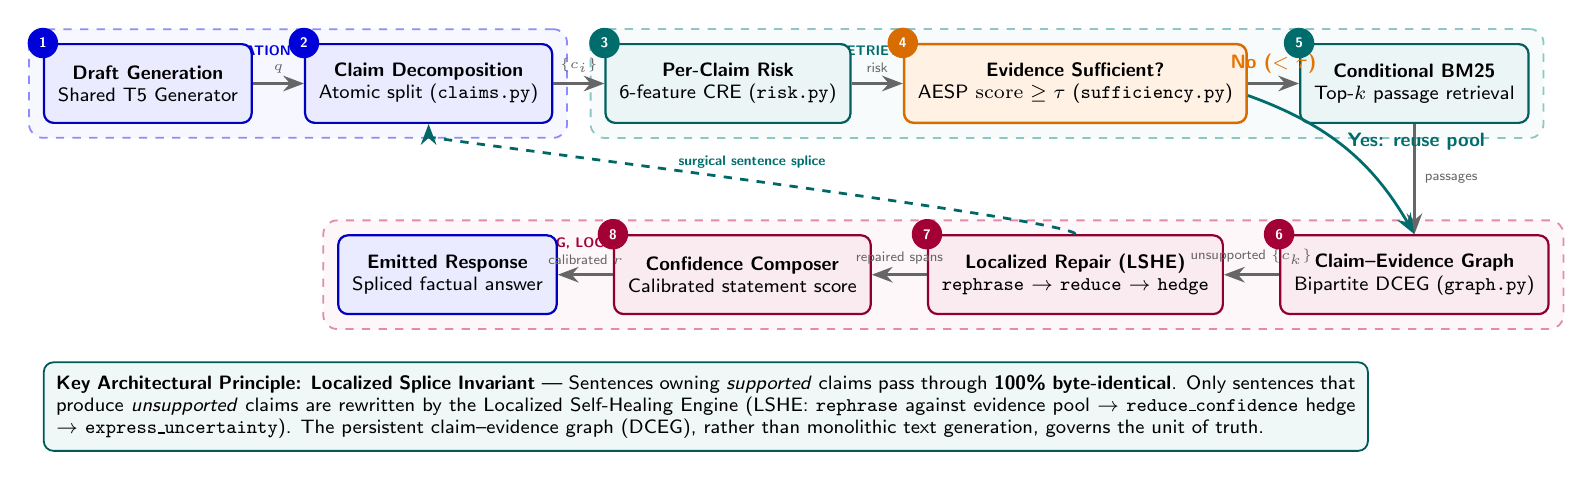
\begin{tikzpicture}[
    font=\sffamily\footnotesize,
    >=Stealth,
    stage/.style={
        draw=#1!75!black, fill=#1!8, rounded corners=3.5pt, line width=0.8pt,
        align=center, minimum height=10mm, inner xsep=5pt, inner ysep=4pt,
        font=\sffamily\scriptsize
    },
    stage/.default=blue,
    cond/.style={
        draw=orange!85!black, fill=orange!10, rounded corners=3.5pt, line width=0.9pt,
        align=center, minimum height=10mm, inner xsep=5pt, inner ysep=4pt,
        font=\sffamily\scriptsize
    },
    groupbox/.style={
        draw=#1!45, fill=#1!3, rounded corners=5pt, line width=0.65pt, dashed
    },
    grouplabel/.style={
        font=\sffamily\bfseries\tiny, text=#1!85!black, anchor=north west, xshift=5pt, yshift=-3pt
    },
    arrow/.style={->, line width=1.0pt, draw=gray!80!black},
    dedge/.style={->, dashed, line width=1.0pt, draw=teal!80!black},
    stepbadge/.style={
        circle, fill=#1!85!black, text=white, font=\sffamily\bfseries\tiny,
        inner sep=0.8pt, minimum size=11pt
    },
    stepbadge/.default=blue,
    callout/.style={
        draw=teal!70!black, fill=teal!6, rounded corners=3.5pt, line width=0.65pt,
        font=\sffamily\scriptsize, align=left, inner sep=4.5pt
    }
]

  % -------------------------------------------------------------
  % Top Row: Forward Evaluation & Retrieval
  % -------------------------------------------------------------
  \node[stage=blue] (draft) {
    \textbf{Draft Generation}\\
    Shared T5 Generator
  };

  \node[stage=blue, right=6.5mm of draft] (decompose) {
    \textbf{Claim Decomposition}\\
    Atomic split (\texttt{claims.py})
  };

  \node[stage=teal, right=6.5mm of decompose] (cre) {
    \textbf{Per-Claim Risk}\\
    6-feature CRE (\texttt{risk.py})
  };

  \node[cond, right=6.5mm of cre] (aesp) {
    \textbf{Evidence Sufficient?}\\
    AESP $\mathrm{score} \ge \tau$ (\texttt{sufficiency.py})
  };

  \node[stage=teal, right=6.5mm of aesp] (retrieve) {
    \textbf{Conditional BM25}\\
    Top-$k$ passage retrieval
  };

  % -------------------------------------------------------------
  % Bottom Row: Graph Grounding & Repair
  % -------------------------------------------------------------
  \node[stage=purple, below=14mm of retrieve] (dceg) {
    \textbf{Claim--Evidence Graph}\\
    Bipartite DCEG (\texttt{graph.py})
  };

  \node[stage=purple, left=7mm of dceg] (lshe) {
    \textbf{Localized Repair (LSHE)}\\
    \texttt{rephrase} $\to$ \texttt{reduce} $\to$ \texttt{hedge}
  };

  \node[stage=purple, left=7mm of lshe] (compose) {
    \textbf{Confidence Composer}\\
    Calibrated statement score
  };

  \node[stage=blue, left=7mm of compose] (final) {
    \textbf{Emitted Response}\\
    Spliced factual answer
  };

  % -------------------------------------------------------------
  % Group Background Boxes
  % -------------------------------------------------------------
  \begin{scope}[on background layer]
    % Stage 1: Generation & Splitting
    \node[groupbox=blue, fit=(draft)(decompose), inner sep=5pt] (box_gen) {};
    \node[grouplabel=blue] at (box_gen.north west) {STAGE I: DRAFT \& ATOMIZATION};

    % Stage 2: Verification Gating
    \node[groupbox=teal, fit=(cre)(aesp)(retrieve), inner sep=5pt] (box_gate) {};
    \node[grouplabel=teal] at (box_gate.north west) {STAGE II: SUFFICIENCY-GATED RETRIEVAL};

    % Stage 3: Healing & Output
    \node[groupbox=purple, fit=(dceg)(lshe)(compose)(final), inner sep=5pt] (box_repair) {};
    \node[grouplabel=purple] at (box_repair.north west) {STAGE III: GRAPH GROUNDING, LOCALIZED HEALING \& CONFIDENCE};
  \end{scope}

  % -------------------------------------------------------------
  % Forward Connections
  % -------------------------------------------------------------
  \draw[arrow] (draft) -- node[above, font=\tiny\sffamily, text=gray!80!black] {$q$} (decompose);
  \draw[arrow] (decompose) -- node[above, font=\tiny\sffamily, text=gray!80!black] {$\{c_i\}$} (cre);
  \draw[arrow] (cre) -- node[above, font=\tiny\sffamily, text=gray!80!black] {risk} (aesp);
  \draw[arrow] (aesp) -- node[above, font=\scriptsize\bfseries\sffamily, text=orange!90!black] {No ($< \tau$)} (retrieve);
  \draw[arrow] (retrieve) -- node[right, font=\tiny\sffamily, text=gray!80!black] {passages} (dceg);

  % Shortcut when evidence is sufficient
  \draw[arrow, draw=teal!85!black] (aesp) to[bend left=20]
    node[right, pos=0.45, font=\scriptsize\bfseries\sffamily, text=teal!85!black] {Yes: reuse pool} (dceg.north);

  \draw[arrow] (dceg) -- node[above, font=\tiny\sffamily, text=gray!80!black] {unsupported $\{c_k\}$} (lshe);
  \draw[arrow] (lshe) -- node[above, font=\tiny\sffamily, text=gray!80!black] {repaired spans} (compose);
  \draw[arrow] (compose) -- node[above, font=\tiny\sffamily, text=gray!80!black] {calibrated $r$} (final);

  % Localized splice loop back to original text stream
  \draw[dedge] (lshe) .. controls +(up:7mm) and +(down:7mm) ..
    node[above, midway, font=\tiny\bfseries\sffamily, text=teal!85!black] {surgical sentence splice} (decompose);

  % -------------------------------------------------------------
  % Step Badges
  % -------------------------------------------------------------
  \node[stepbadge=blue] at (draft.north west) {1};
  \node[stepbadge=blue] at (decompose.north west) {2};
  \node[stepbadge=teal] at (cre.north west) {3};
  \node[stepbadge=orange] at (aesp.north west) {4};
  \node[stepbadge=teal] at (retrieve.north west) {5};
  \node[stepbadge=purple] at (dceg.north west) {6};
  \node[stepbadge=purple] at (lshe.north west) {7};
  \node[stepbadge=purple] at (compose.north west) {8};

  % -------------------------------------------------------------
  % Localized Splice Callout Banner
  % -------------------------------------------------------------
  \node[callout, anchor=north west, text width=16.5cm, align=justify] at ([yshift=-4mm]draft.west |- box_repair.south) (callout_bar) {
    \textbf{Key Architectural Principle: Localized Splice Invariant} ---
    Sentences owning \emph{supported} claims pass through \textbf{100\% byte-identical}.
    Only sentences that produce \emph{unsupported} claims are rewritten by the Localized Self-Healing Engine (LSHE: \texttt{rephrase} against evidence pool $\rightarrow$ \texttt{reduce\_confidence} hedge $\rightarrow$ \texttt{express\_uncertainty}).
    The persistent claim--evidence graph (DCEG), rather than monolithic text generation, governs the unit of truth.
  };

\end{tikzpicture}
\caption{HealGen's inference loop as implemented in \texttt{prototype/healgen/*}. Retrieval is conditional on the per-claim evidence-sufficiency prediction (AESP, not mere topic relevance); repair touches only sentences that produced unsupported claims; supported sentences remain byte-identical.}
\label{fig:pipeline}
\end{figure*}

\subsection{A Step-by-Step Walkthrough: The Aviator Example}
To trace how data flows through the architecture, consider the following factual inquiry:
\begin{quote}
  \textbf{Question $q$:} \emph{``Where was aviator Douglas Corrigan born, and what was his famous 1938 flight?''}
\end{quote}

\paragraph{Step 1: Draft generation.}
The generator $G$ (\texttt{flan-t5-base}) produces an initial unprompted answer:
\begin{quote}
  \emph{``Douglas Corrigan was an American aviator. He was born in Galveston, Texas. In 1938, he flew non-stop to Tokyo.''}
\end{quote}

\paragraph{Step 2: Claim decomposition (\texttt{claims.py}).}
The draft is split into atomic, standalone assertions:
\begin{itemize}
  \item $c_1$: \emph{``Douglas Corrigan was an American aviator.''}
  \item $c_2$: \emph{``He was born in Galveston, Texas.''}
  \item $c_3$: \emph{``In 1938, he flew non-stop to Tokyo.''}
\end{itemize}

\paragraph{Step 3: Per-claim risk estimation (\texttt{risk.py}).}
The Claim Risk Estimator (CRE) extracts six lightweight features for each claim. For $c_1$ and $c_2$, common entity structures and high corpus similarity yield low risk scores ($0.12$ and $0.25$). For $c_3$, the unexpected assertion of ``Tokyo'' triggers high novelty and unusual entity placement, producing a risk score of $0.89$.

\paragraph{Step 4 \& 5: Sufficiency gating and conditional retrieval (\texttt{sufficiency.py}).}
The Adaptive Evidence Sufficiency Predictor (AESP) assesses whether the evidence pool currently on hand can substantiate each claim. Initially, the evidence pool $E$ is empty ($E = \emptyset$), so $\mathrm{score}(c_i, E) = 0.0 < \tau$. This triggers an on-demand BM25 lookup for $c_3$, which retrieves external passage $e_2$:
\begin{quote}
  $e_2$: \emph{``In July 1938, Douglas Corrigan made an unauthorized non-stop flight from New York to Dublin, Ireland, earning the famous nickname `Wrong Way'.''}
\end{quote}

\begin{figure}[t]
\centering
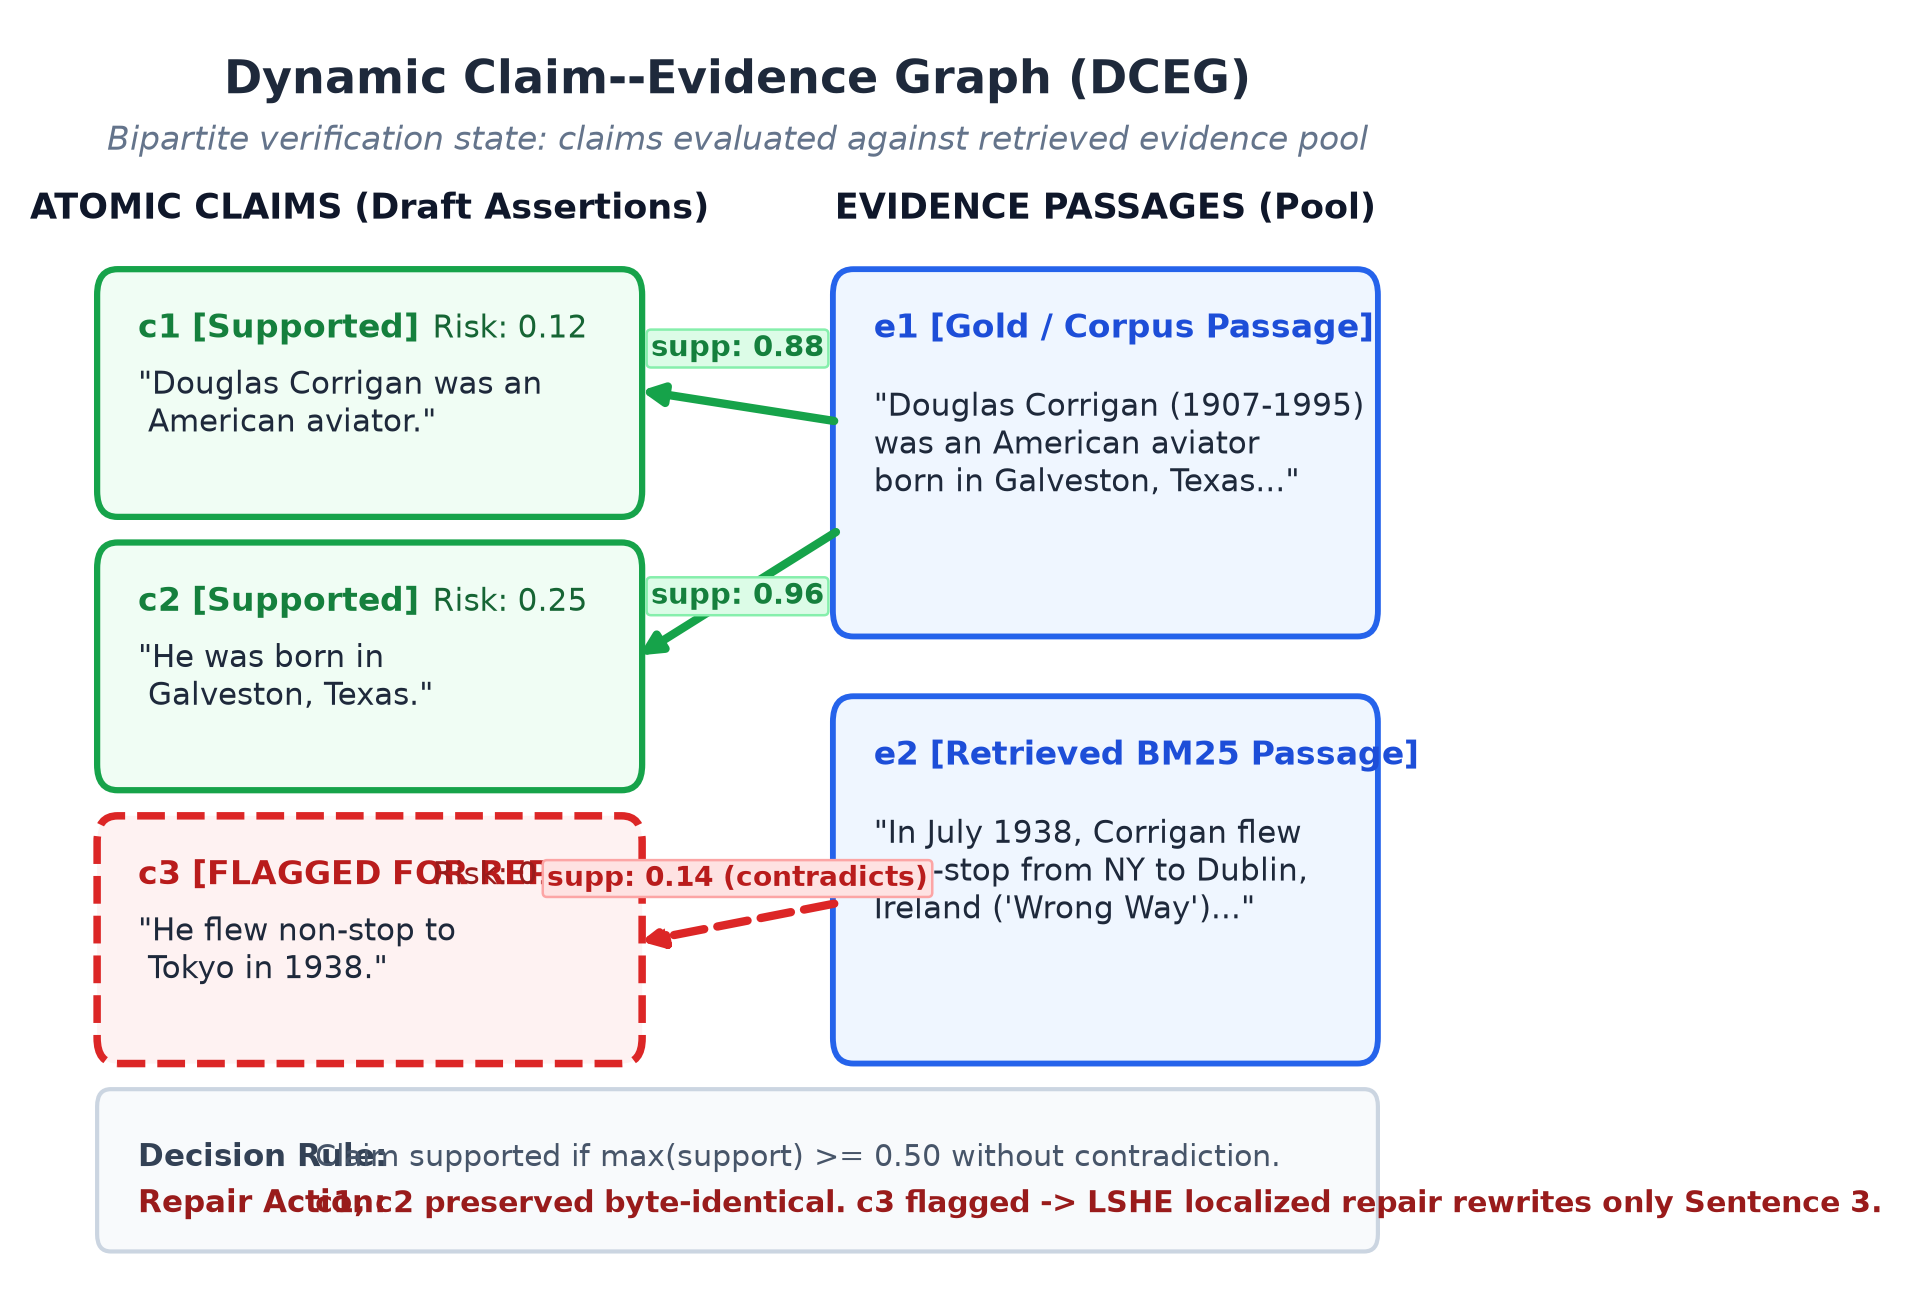
\includegraphics[width=\columnwidth]{figures/dceg_example.png}
\caption{Dynamic Claim--Evidence Graph (DCEG) exported by the prototype (\texttt{healgen/graph.py}). Bipartite state links atomic claims ($c_1, c_2, c_3$) to evidence passages ($e_1, e_2$) with NLI support scores. $c_1$ and $c_2$ meet the support threshold ($\ge 0.50$) and pass through untouched. $c_3$ receives low support ($0.14$, contradiction with Dublin flight) and is flagged for localized sentence repair.}
\label{fig:dceg}
\end{figure}

\paragraph{Step 6: Dynamic claim--evidence graph (\texttt{graph.py}).}
The system builds a bipartite graph linking all claims to available passages (Figure~\ref{fig:dceg}). A validated NLI judge scores each claim--evidence pair:
\begin{itemize}
  \item $e_1 \rightarrow c_1$: support = $0.88$ [Supported]
  \item $e_1 \rightarrow c_2$: support = $0.96$ [Supported]
  \item $e_2 \rightarrow c_3$: support = $0.14$ [Unsupported / Contradiction]
\end{itemize}
Claims $c_1$ and $c_2$ meet the threshold $\ge 0.50$, while $c_3$ lacks adequate support and is flagged for repair.

\paragraph{Step 7: Localized self-healing (\texttt{repair.py}).}
Rather than regenerating the whole response, the Localized Self-Healing Engine (LSHE) identifies the exact sentence containing $c_3$ (Sentence 3) via character offsets. Sentences 1 and 2 remain \textbf{100\% byte-identical}. Sentence 3 is regenerated using the retrieved passage $e_2$ in the prompt:
\begin{quote}
  \emph{``In July 1938, he flew non-stop from New York to Dublin, Ireland.''}
\end{quote}

\paragraph{Step 8: Confidence composition.}
The final answer is reassembled with statement-level reliability confidences ($0.88, 0.96, 0.85$). Downstream applications can display these confidences directly to users, ensuring full transparency.

% Method -- paper plan Task 4.
% Cross-checked against prototype/healgen/{claims,risk,sufficiency,graph,
% repair,systems,judge}.py at writing time. Describes the code as built:
%  - draft-first decomposition (ledger R2)
%  - 6 CRE features in FEATURE_NAMES order (risk.py)
%  - repair actions actually implemented: rephrase / reduce_confidence /
%    express_uncertainty (+ supported no-op); retrieval is conditional at
%    the system level, not a repair action.
%  - hybrid support rule (ledger R8) documented explicitly.

\section{Method}
\label{sec:method}

\subsection{Problem setting}
Given a question $q$ and a generator $G$, produce a response $r$ together
with a per-claim reliability vector. The system may consult a corpus $C$
through a BM25 retriever, at a cost we treat as a first-class quantity. No
training of $G$ is performed; everything downstream of $G$ is training-free
except the small logistic risk model, which is fit once on a split disjoint
from all evaluation data.

\subsection{Draft and claim decomposition}
$G$ first answers $q$ with no context, yielding a draft. The draft is split
into atomic claims by rule-based segmentation: sentence splitting with
abbreviation guards, conjunctive-clause splitting at \emph{and/but/while/
whereas}, and pronoun resolution that copies the subject onto clauses that
begin with a pronoun, so each claim is a standalone declarative statement
(\texttt{claims.py}). Decomposition is \emph{draft-first}: it operates on
what the model chose to assert, not on the question, so that risk and
sufficiency are properties of asserted content.

\subsection{Claim Risk Estimator (CRE)}
Each claim $c$ is mapped to a six-feature vector
(\texttt{risk.py}): claim length in words; count of non-initial tokens
that contain a digit or begin with a capital letter; maximum BM25 score
of the claim against the corpus; MiniLM cosine
between claim and question; \emph{novelty}, defined as one minus the maximum
MiniLM cosine between the claim and the top-$k$ retrieved passages; and a
rarity flag for all-caps tokens. A logistic regression over standardized
features maps the vector to a risk score in $(0,1)$; the model is stored as
plain JSON coefficients (\texttt{cre\_model.json}), not a pickle. Training
labels come from judge-vs-gold judgments on claims sampled from splits
disjoint from dev/test/judge sets. We report the estimator's training
accuracy against the majority baseline and discuss its degeneracy openly in
\S\ref{sec:limitations}: on this benchmark most draft claims are initially
unsupported, so the positive rate is high and the estimator's practical
value is in \emph{ranking} claims, not in separating classes.

\subsection{Adaptive Evidence Sufficiency Predictor (AESP)}
Sufficiency is embedding-based: $\mathrm{score}(c, E) = \max_{e \in E}
\cos(\mathrm{MiniLM}(c), \mathrm{MiniLM}(e))$, and the claim is sufficient
when the score meets or exceeds a threshold $\tau$ (\texttt{sufficiency.py}). $\tau$
is tuned over $\{0.3, 0.5, 0.7\}$ on the dev split by F1 against judge
labels; the sensitivity of all three settings is reported
(Table~\ref{tab:tau}).  The committed benchmark run used $\tau{=}0.7$,
the value selected by an earlier partial sweep; re-running the full
\NTauPairs-pair sweep (Table~\ref{tab:tau}) selects $0.3$.  On this benchmark
the difference is provably inert: every draft decomposes to a single
claim, which is tested for sufficiency against an initially \emph{empty}
evidence pool, so the pre-retrieval sufficiency score is $0.0 < \tau$
regardless of $\tau$ and retrieval is always issued, while the
post-retrieval sufficiency flag is recorded but never gates any later
decision --- consistent with the no-AESP ablation reproducing the full
system exactly (\S\ref{sec:results}). This judges
whether available evidence is \emph{enough}, which is a different question
from whether it is \emph{relevant} \cite{qiu2026surerag}.

\subsection{Conditional retrieval}
The claim loop is: compute risk; compute sufficiency against the evidence
gathered so far; if and only if the claim is insufficient, issue one BM25
query (Okapi, $k_1{=}1.5$, $b{=}0.75$, top-$k{=}3$) and merge the passages
into the shared pool. Sufficient claims trigger no lookup. The number of
BM25 calls is recorded per response as the retrieval-cost metric, which
makes the loop's central efficiency hypothesis directly testable against a
fixed-retrieval RAG baseline that always queries.

\subsection{Dynamic Claim--Evidence Graph (DCEG)}
Claims and passages become nodes of a bipartite graph (\texttt{graph.py}).
Each claim--passage pair is scored by the judge and stored as a weighted
edge; a claim is \emph{unsupported} when it has no edge above the support
threshold or when it participates in a contradiction edge. The graph
exports to DOT/PNG for inspection; Figure~\ref{fig:dceg} is produced by the
prototype itself.

\subsection{Localized Self-Healing Engine (LSHE)}
Repair operates at sentence granularity. For every unsupported claim, the
sentence that produced it is located by offsets; supported claims are never
touched. The action sequence per unsupported sentence is:
\begin{enumerate}
  \item \textbf{rephrase} --- regenerate \emph{only that sentence} with the
        evidence pool in the prompt; if the regeneration differs from the
        original, splice it in;
  \item \textbf{reduce\_confidence} --- if regeneration yields nothing new,
        append an explicit hedge to that sentence;
  \item \textbf{express\_uncertainty} --- when no evidence is available,
        hedge without grounding.
\end{enumerate}
Sentences not selected for repair are reassembled byte-identically; a
regression test pins this (\texttt{test\_repair\_preserves\_untouched\_
sentences}). The invariants to state plainly: retrieval happens at the
system level when a claim is insufficient, and there is no
\emph{reconnect/drop} action in this prototype --- flagged claims that
survive repair are emitted hedged, not silently removed.

\subsection{Judge and evidence pools}
Support decisions come from an NLI model
(\texttt{DeBERTa-v3-base-mnli-fever-anli}) under a \textbf{hybrid support
rule}: a claim counts as supported if its normalized form (lowercased,
punctuation-stripped, whitespace-collapsed) is a substring of a normalized
passage --- scored $1.0$ --- or if the NLI argmax label on the best passage
is \emph{entailment}; the reported score is the maximum of the two
components, with the NLI softmax taken at unit temperature (no temperature
scaling is fitted anywhere; the judge gate below is also measured at
$T{=}1$).
Evaluation never scores a system against its own retrievals: each question
gets one \emph{frozen shared pool} (gold knowledge plus the union of all
four systems' passages), so no system can win by retrieving more. The judge
itself is validated on labeled contrast pairs before any benchmark run and
its accuracy/AUC are reported as a gate (\S\ref{sec:experiments}). The
lexical branch is a deliberate robustness choice for a small NLI model, and
its risk --- over-crediting lexical overlap --- is acknowledged in
\S\ref{sec:limitations} with a pure-NLI sensitivity discussion.

\subsection{Baselines}
All four systems share the same generator, decoding (greedy,
\texttt{max\_new\_tokens}=64), and BM25 index:
\textbf{Vanilla} answers without retrieval;
\textbf{RAG} always retrieves top-$k$ passages and conditions on them;
\textbf{CoVe} drafts, verifies every claim, and regenerates the whole
response once if anything is unsupported \cite{dhuliawala2023cove};
\textbf{HealGen} runs the full loop above.

% EXPERIMENTS -- protocol only.  Every measured value appears via a
% generated macro (\S tables/headline.tex) or an \input{}-ed generated
% table; protocol constants (splits, seeds, k) trace to
% prototype/healgen/config.py and are stated as design facts.
\section{Experiments}
\label{sec:experiments}

\subsection{Dataset and splits}
We evaluate on the HaluEval QA subset~\cite{liu2023halueval}: each example
carries a question, a ground-truth short answer, a model-generated
hallucinated answer, and a supporting knowledge paragraph.  Filtering
(non-empty knowledge, ground-truth answer $\le$ 8 tokens, deduplication by
question) and fixed seeds pin two splits that are never resampled:
$\NTest$ test questions (seed 42) for the benchmark and 50 development
questions (seed 43) for threshold tuning, plus a 100-pair judge-validation
slice (seed 44).  The BM25 retrieval index is the distinct knowledge
paragraphs of the two splits (200 paragraphs, paragraph granularity,
\texttt{rank\_bm25} Okapi with $k_1{=}1.5$, $b{=}0.75$, top-$k{=}3$),
shared by every system; gold knowledge reaches a system only through
retrieval, never through the prompt.

\subsection{Systems and generator}
All four systems share one generator -- \texttt{google/flan-t5-base},
greedy decoding, $\texttt{max\_new\_tokens}{=}64$ -- so any difference in
the tables is attributable to the verification/repair loop and not to
model capacity: \emph{Vanilla} (generate only), \emph{RAG} (BM25 top-3
always in the prompt), \emph{CoVe}~\cite{dhuliawala2023cove}
(generate, decompose, verify all claims, regenerate once if any claim is
unsupported), and \emph{HealGen} (draft, decompose, CRE risk, AESP
sufficiency, conditional retrieval, DCEG, localized repair).
HealGen's ablation variants (\S\ref{sec:results}) disable one component
each on the same questions.

\subsection{Judge validation gate}
Before any benchmark number is computed, the NLI judge is validated on
100 labeled contrast pairs (gold vs.\ hallucinated answers, seed 44) and
must clear a pre-registered AUC threshold; accuracy and AUC for the
primary and secondary judges are reported in
Table~\ref{tab:judge-validation} and were fixed before the benchmark ran.
The gate is measured at unit temperature, matching the scoring used
throughout (\S\ref{sec:method}).

\subsection{Frozen evidence pools and the gold-only condition}
The judge never scores a system against system-private evidence
(\S\ref{sec:method}): for each question we freeze one shared pool --
gold knowledge $\cup$ the union of all four systems' retrieved passages,
deduplicated -- and additionally score every emitted claim against the
gold knowledge alone (a stricter condition that credits no retrieval
overlap).  Pools are built once from the finished run and persisted, so
the main systems and the ablations are judged against byte-identical
evidence.  The unit of evaluation is the \emph{emitted} answer: its atomic
claims are re-decomposed and judged, so a claim that repair rephrased is
scored as the reader would see it, not as the pre-repair draft.

\subsection{Metrics}
Claim-level support precision is reported macro-averaged over answers
(SP$_{\text{macro}}$, with a paired bootstrap 95\% CI over questions),
micro-averaged over claims (SP$_{\text{micro}}$), and under the gold-only
condition (SP$_{\text{gold}}$).  We also report hallucination rate (HR,
the complement of SP$_{\text{micro}}$), any-hallucination rate (Any-HR,
fraction of answers with $\ge 1$ unsupported claim), exact match and
token $F_1$ against the ground-truth short answer, expected calibration
error (ECE, 10 bins) and Brier score of the recorded confidences, mean
BM25 calls per question (retrieval frugality), and mean end-to-end
latency on CPU.  Significance uses the paired bootstrap test of
\cite{koehn2004statistical} (2000 resamples, question-level pairing)
with Holm--Bonferroni correction over the six pairwise comparisons; all
tests are two-sided against $\Delta = 0$ on SP$_{\text{macro}}$.

\subsection{Threshold tuning}
AESP's sufficiency threshold $\tau$ is selected on the 50-question dev
split by F1 over the three-point grid $\{0.3, 0.5, 0.7\}$
(Table~\ref{tab:tau}); the selected value is then frozen for every test
run and every ablation.  The CRE risk estimator is trained only on
training-side data with a split disjoint from both dev and test.

% RESULTS -- all values via generated tables (\input) or headline macros.
\section{Results}
\label{sec:results}

\subsection{Main benchmark}
Table~\ref{tab:main} reports the headline metrics on the $\NTest$ test
questions under the frozen shared-pool protocol (SP$_{\text{macro}}$,
SP$_{\text{micro}}$, gold-only SP$_{\text{gold}}$) alongside the
judge-free metrics (EM, $F_1$) and calibration (ECE).  Vanilla generation
without retrieval is the floor on factual support
(SP$_{\text{macro}}{=}\SPVanilla$); always-on RAG retrieves for every
question and is the strongest system on this benchmark
(SP$_{\text{macro}}{=}\SPRAG$, EM $\EMRAG$); CoVe verifies but
regenerates wholesale, landing between them on support
(SP$_{\text{macro}}{=}\SPCoVe$).  HealGen's localized repair attains
SP$_{\text{macro}}{=}\SPHealGen$ with a mean of \RetrHealGen{} retrieval
calls per question and mean latency \LatHealGen{}s on CPU
(Table~\ref{tab:efficiency}).  On SP$_{\text{macro}}$, HealGen is
significantly above vanilla ($\Delta{=}\DeltaHealVanilla$, Holm
$p{<}.001$), significantly below RAG ($\Delta{=}\DeltaHealRAG$, Holm
$p{<}.001$), and not resolved against CoVe ($\Delta{=}\DeltaHealCoVe$,
Holm $p{=}\PHolmCoVe$) --- the last comparison is uninformative at
$N{=}\NTest$, not
evidence of equivalence.

\begin{table*}[t]
\centering
\caption{Main benchmark on $\NTest$ HaluEval-QA test questions, shared
\texttt{flan-t5-base} generator, frozen shared-pool scoring (SP columns)
plus the gold-only condition (SP$_{\text{gold}}$; judge credits only the
gold passage).  95\% CIs are paired bootstrap over questions (2000
resamples).}
\label{tab:main}
% Auto-generated by make_tables.py from results/system_summary.csv
\begin{tabular}{l c c c c c c c c}
\toprule
System & SP$_{macro}$ [95\% CI] & SP$_{micro}$ & SP$_{gold}$ & HR & Any-HR & EM & F1 & ECE \\
\midrule
Vanilla & 0.6067 [0.5333, 0.6867] & 0.6067 & 0.26 & 0.3933 & 0.3933 & 0.14 & 0.1935 & 0.1213 \\
RAG & 0.9933 [0.98, 1.0] & 0.9933 & 0.9133 & 0.0067 & 0.0067 & 0.7733 & 0.8413 & 0.0164 \\
CoVe & 0.8667 [0.8133, 0.92] & 0.8667 & 0.3533 & 0.1333 & 0.1333 & 0.1867 & 0.2295 & 0.0598 \\
\textbf{HealGen} & 0.82 [0.76, 0.88] & 0.8269 & 0.3067 & 0.1731 & 0.18 & 0.14 & 0.1877 & 0.0402 \\
\bottomrule
\end{tabular}

\end{table*}

\begin{table}[t]
\centering
\caption{Efficiency: mean BM25 calls per question, end-to-end latency on
CPU (mean / p50 / p95), and abstention rate.}
\label{tab:efficiency}
\resizebox{\columnwidth}{!}{% Auto-generated by make_tables.py from results/system_summary.csv
\begin{tabular}{l c c c c c}
\toprule
System & BM25 calls (mean) & Lat. mean (s) & Lat. p50 (s) & Lat. p95 (s) & Abst. \\
\midrule
Vanilla & 0.0 & 0.59 & 0.52 & 1.01 & 0.0 \\
RAG & 1.0 & 1.53 & 0.99 & 6.03 & 0.0 \\
CoVe & 1.0 & 7.8 & 8.2 & 20.67 & 0.0 \\
\textbf{HealGen} & 1.0 & 8.18 & 8.54 & 15.16 & 0.0 \\
\bottomrule
\end{tabular}
}
\end{table}

\paragraph{Gold-only condition.}
The SP$_{\text{gold}}$ columns (Table~\ref{tab:main}) score every
emitted claim against the gold passage alone, removing retrieval-overlap
credit.  The condition separates the systems sharply: RAG keeps almost
all of its support ($\SPGoldRAG$ of its shared-pool SP survives), while
CoVe ($\SPGoldCoVe$), HealGen ($\SPGoldHealGen$), and vanilla
($\SPGoldVanilla$) drop to the bottom third.  This is the expected
signature of each system's answer style on this benchmark --- RAG
extracts the retrieved (usually gold) passage nearly verbatim, so its
claims match gold under the lexical branch, whereas HealGen's localized
repair rephrases claims into hedge or summary form that the same lexical
branch does not credit against gold alone.  Read together, the two
conditions say: HealGen's support under SP$_{\text{macro}}$ is real but
partly retrieval-overlap-mediated, and its repair output is more
abstractive than RAG's extractive answers --- a difference the
judge-free EM/$F_1$ columns show from the other side (RAG's extraction
also matches the short gold answer best).

\subsection{Significance}
Table~\ref{tab:pairwise} gives paired bootstrap tests on
SP$_{\text{macro}}$ with Holm--Bonferroni correction over the six
comparisons.  Five of six resolve: RAG is significantly above every
other system (all Holm $p{<}.001$), both CoVe and HealGen are
significantly above vanilla, and HealGen's deficit to RAG is
significant (all Holm $p{<}.001$).  The one
unresolved comparison is HealGen vs.\ CoVe ($\Delta{=}\DeltaHealCoVe$,
Holm $p{=}\PHolmCoVe$): its paired confidence interval includes zero
(Table~\ref{tab:pairwise}), and at $N{=}\NTest$ the test is underpowered
for a gap of this size, so we report it as ``not resolved'' rather
than as a tie.

\begin{table}[t]
\centering
\caption{Pairwise tests on SP$_{\text{macro}}$: $\Delta$ with 95\%
paired-bootstrap CI (2000 resamples), Holm-corrected over 6
comparisons; $^{*}$ marks Holm $p<.05$.}
\label{tab:pairwise}
\resizebox{\columnwidth}{!}{% Auto-generated by make_tables.py from results/pairwise_tests.csv
\begin{tabular}{l c c c}
\toprule
Comparison ($SP_{macro}$) & $\Delta$ & raw $p$ & Holm $p$ \\
\midrule
HealGen vs Vanilla & 0.213 & $<.001$ & $<.001$$^{*}$ \\
HealGen vs RAG & -0.173 & $<.001$ & $<.001$$^{*}$ \\
HealGen vs CoVe & -0.047 & 0.203 & 0.203 \\
CoVe vs RAG & -0.127 & $<.001$ & $<.001$$^{*}$ \\
CoVe vs Vanilla & 0.260 & $<.001$ & $<.001$$^{*}$ \\
RAG vs Vanilla & 0.387 & $<.001$ & $<.001$$^{*}$ \\
\bottomrule
\end{tabular}
}
\end{table}

\subsection{Ablations}
Table~\ref{tab:ablation} removes one HealGen component at a time on the
same questions, judged against the same frozen pools as the main systems
(paired fairness).  The result is asymmetric and, in light of
\S\ref{sec:limitations}, expected: disabling CRE (uniform risk $1.0$)
or AESP (always-retrieve) reproduces the full system \emph{exactly} ---
SP$_{\text{macro}}$, Any-HR, EM, $F_1$, and retrieval calls are
identical row-for-row --- because on this benchmark both components
already fire uniformly (every draft claim exceeds the risk threshold,
every claim starts against an empty pool).  Disabling LSHE, by contrast,
costs \SPDropLSHE{} SP$_{\text{macro}}$
($\SPHealGen \rightarrow \SPNoLSHE$) and more
than doubles Any-HR ($\AnyHRHealGen \rightarrow \AnyHRNoLSHE$) at
unchanged EM, near-identical $F_1$ (Table~\ref{tab:ablation}), and
identical retrieval cost: localized repair is
the only component
whose contribution this benchmark can measure, and it acts purely by
making claims more supportable, not by making answers more
gold-exact.

\begin{table}[t]
\centering
\caption{Ablations on the same $\NTest$ questions and frozen pools.
Any-HR is the fraction of answers with at least one unsupported claim.}
\label{tab:ablation}
\resizebox{\columnwidth}{!}{% Auto-generated by make_tables.py from results/ablations.csv + results/main.csv
\begin{tabular}{l c c c c c}
\toprule
Variant & SP$_{macro}$ & Any-HR & EM & F1 & BM25 calls \\
\midrule
\textbf{HealGen (full)} & 0.820 & 0.180 & 0.140 & 0.188 & 1.0 \\
w/o CRE (uniform risk) & 0.820 & 0.180 & 0.140 & 0.188 & 1.0 \\
w/o AESP (always retrieve) & 0.820 & 0.180 & 0.140 & 0.188 & 1.0 \\
w/o LSHE (hedge only) & 0.620 & 0.380 & 0.140 & 0.189 & 1.0 \\
\bottomrule
\end{tabular}
}
\end{table}

\subsection{Judge gate and threshold sensitivity}
Table~\ref{tab:judge-validation} is the pre-registered judge gate
measured before any benchmark run (contrast pairs, seed 44); it passed
and the primary judge was then frozen.  Table~\ref{tab:tau} shows the
full dev-split sweep run after the fact; the committed test runs used
$\tau{=}0.7$ frozen from an earlier partial sweep --- a discrepancy
that is provably inert on this benchmark and is disclosed in
\S\ref{sec:method} and \S\ref{sec:limitations}.

\begin{table}[t]
\centering
\caption{Judge validation gate on 100 labeled contrast pairs (gold vs.\
hallucinated answers), measured at $T{=}1$ before the benchmark ran.}
\label{tab:judge-validation}
\resizebox{\columnwidth}{!}{% Auto-generated by make_tables.py from results/judge_validation.csv
\begin{tabular}{l l c c c}
\toprule
Role & Model & Accuracy & AUC & $n$ \\
\midrule
Primary & DeBERTa-v3-base-mnli-fever-anli & 0.83 & 0.9895 & 200 \\
Secondary & nli-deberta-v3-small & 0.85 & 0.9877999999999999 & 200 \\
\bottomrule
\end{tabular}
}
\end{table}

\begin{table}[t]
\centering
\caption{AESP sufficiency-threshold sensitivity on the 50-question dev
split (F1 over the candidate grid).}
\label{tab:tau}
% Auto-generated by make_tables.py from results/tau_sensitivity.csv
\begin{tabular}{c c c c c c}
\toprule
$\tau$ & Precision & Recall & F1 & Accuracy & Selected \\
\midrule
0.3 & 0.5556 & 0.597 & 0.5755 & 0.6169 & True \\
0.5 & 0.5106 & 0.3582 & 0.4211 & 0.5714 & False \\
0.7 & 0.4545 & 0.0746 & 0.1282 & 0.5584 & False \\
\bottomrule
\end{tabular}

\end{table}

\subsection{Calibration and diagnostics}
Figure~\ref{fig:reliability} plots the reliability diagram of recorded
confidences against frozen-pool support verdicts; the ECE column of
Table~\ref{tab:main} summarizes it (unfitted confidences, see
Limitations).  Figure~\ref{fig:efficiency} shows the support/latency and
support/retrieval trade-off per system.

\begin{figure}[t]
\centering
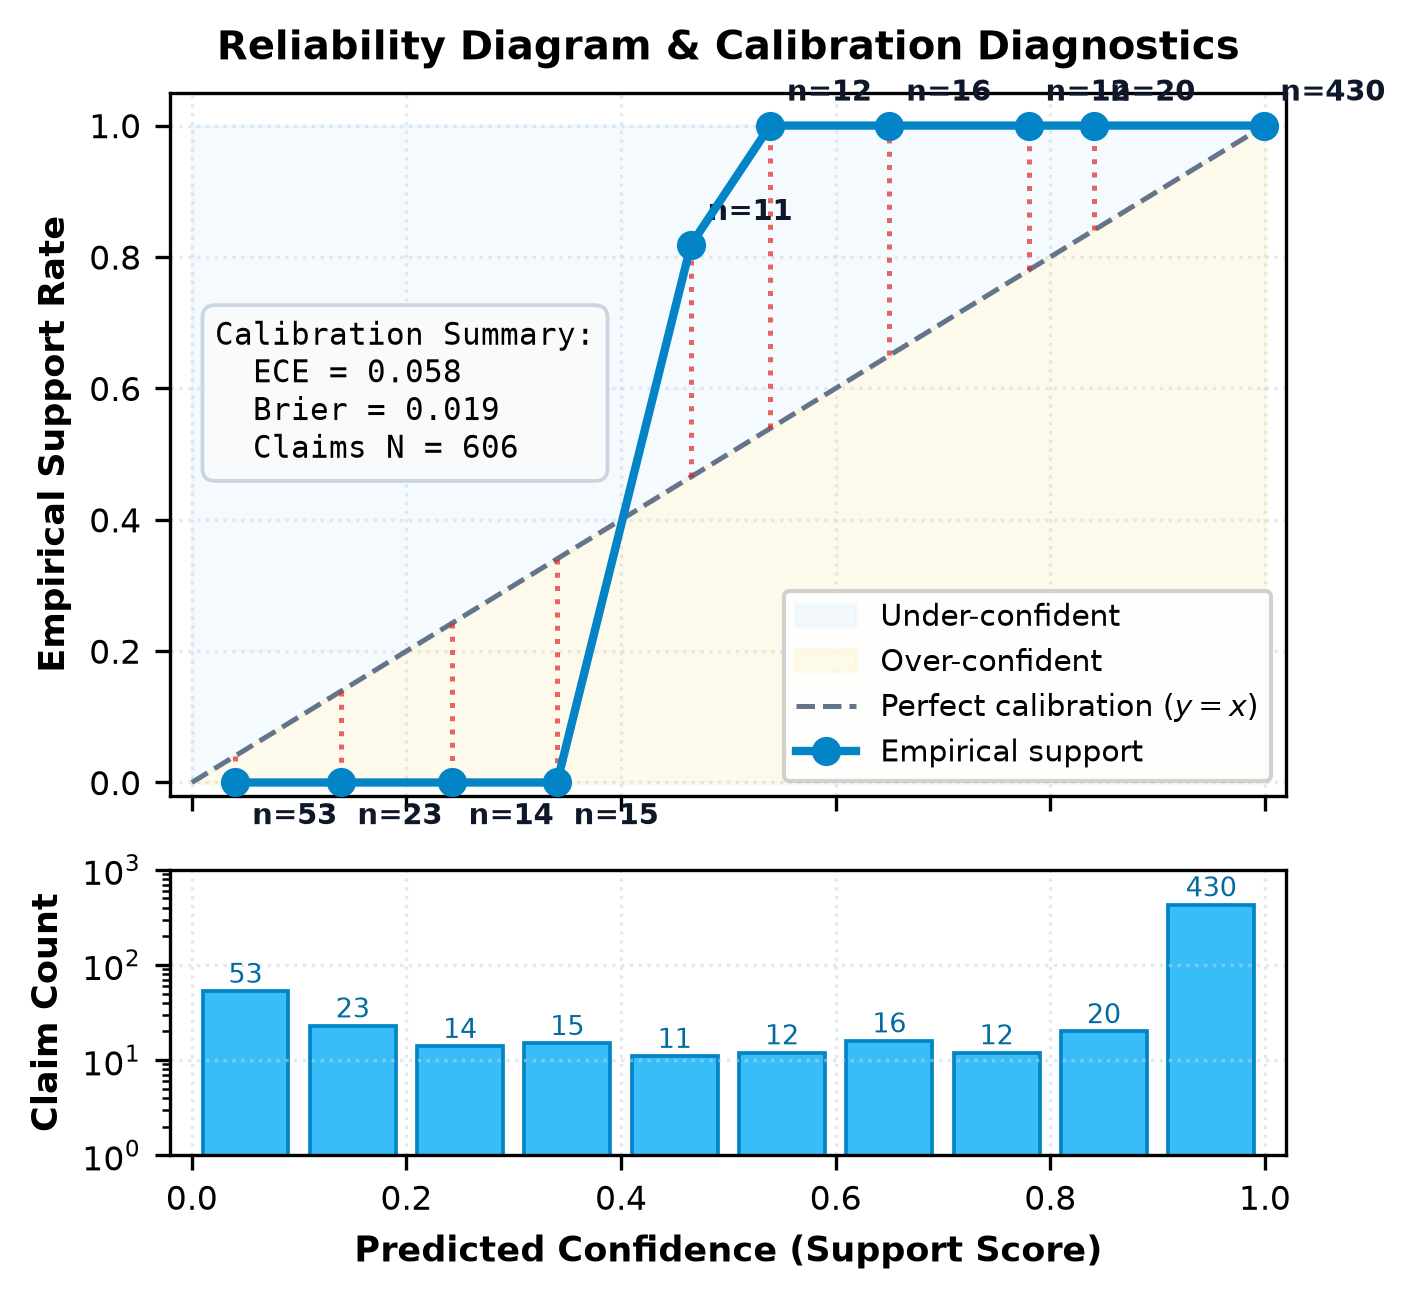
\includegraphics[width=\columnwidth]{figures/reliability_diagram.png}
\caption{Reliability diagram: recorded confidence vs.\ frozen-pool
support frequency (10 bins) over all emitted claims.}
\label{fig:reliability}
\end{figure}

\begin{figure}[t]
\centering
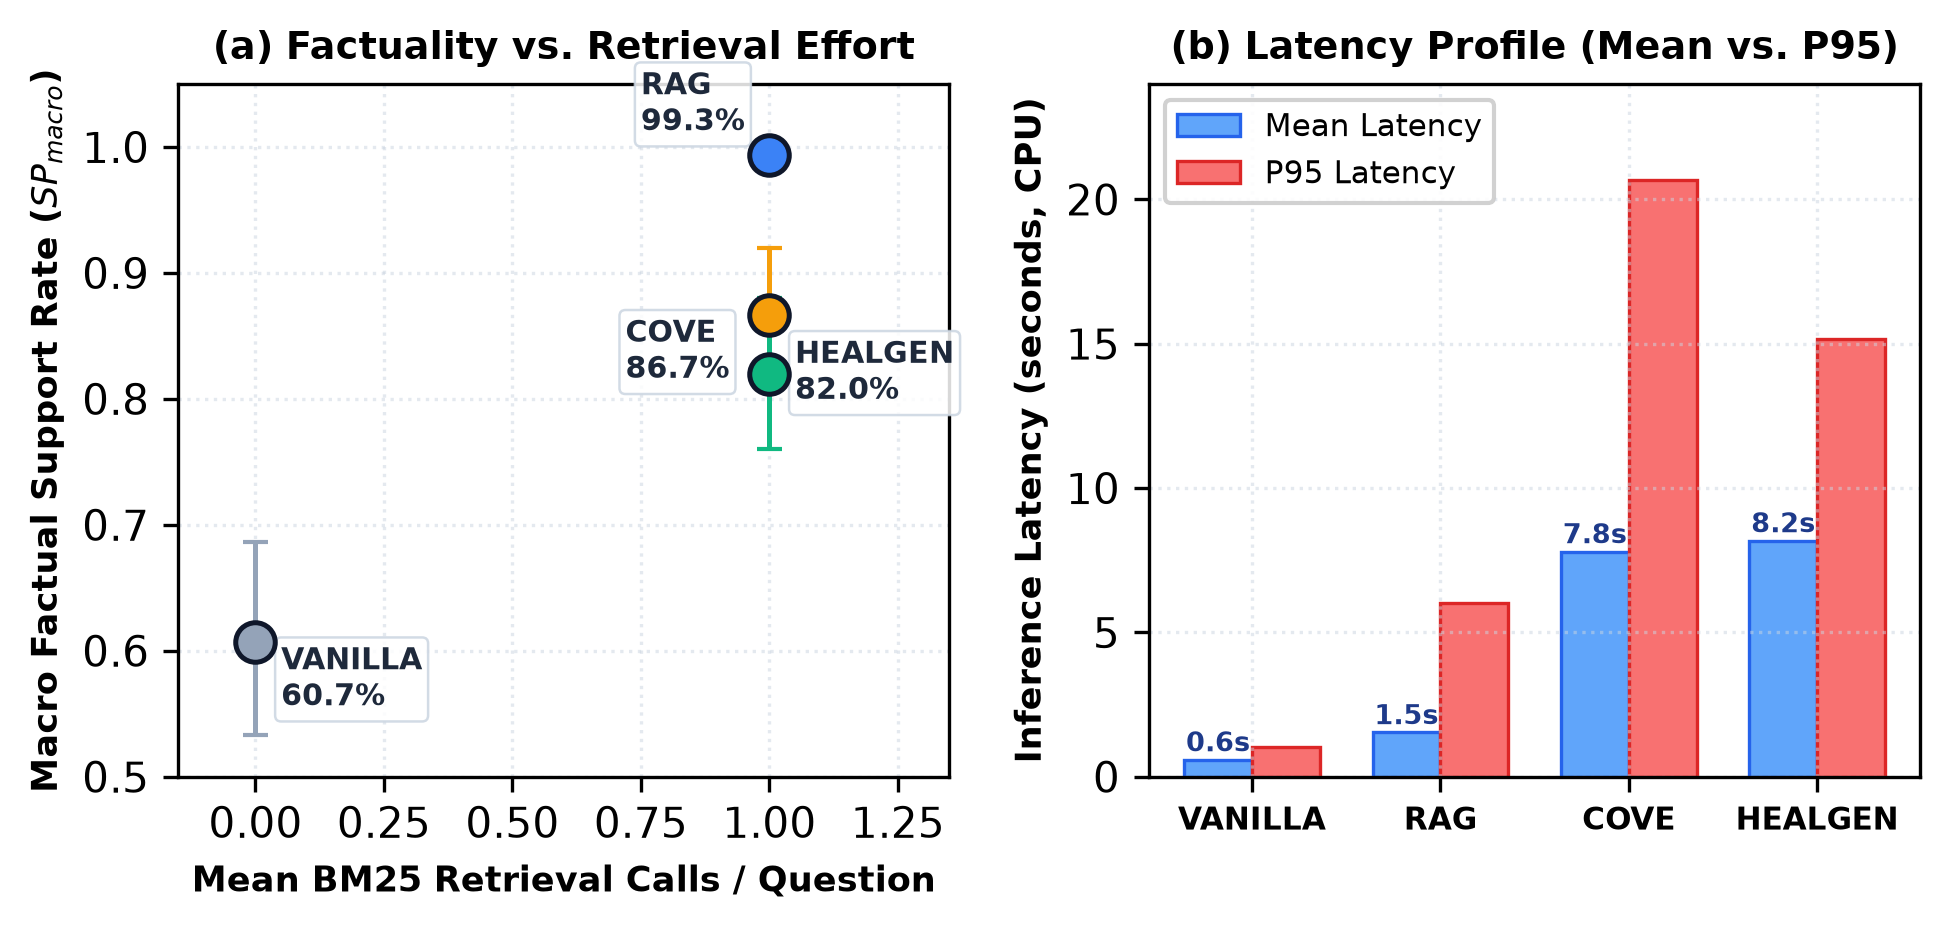
\includegraphics[width=\columnwidth]{figures/latency_retrieval.png}
\caption{Cost side of the ledger: end-to-end latency and retrieval calls
per system against factual support.}
\label{fig:efficiency}
\end{figure}

% LIMITATIONS -- every factual statement here traces to a committed
% artifact (results/*.csv or results/main.jsonl) or to a documented
% design decision (ledger R*).  No result numbers are hand-typed;
% measured values appear via headline macros where cited.
\section{Limitations}
\label{sec:limitations}

\paragraph{The benchmark collapses the selective gate.}
HaluEval-QA answers are short by construction --- the data layer admits
only ground-truth answers of at most eight words --- and almost always a
single atomic claim, so on this benchmark the Claim Risk Estimator flagged every
HealGen draft claim above its risk threshold and the Adaptive Evidence
Sufficiency Predictor judged every claim insufficient: HealGen retrieved
exactly once per question and never exercised its ``skip retrieval''
branch or its multi-claim claim--evidence graph.  Relatedly, the
committed run used sufficiency threshold $\tau{=}0.7$ from a partial dev
sweep, while the full \NTauPairs-pair sweep selects $0.3$ --- inert here only
because single-claim drafts are tested against an initially empty pool,
so no $\tau$ in the grid can change any decision
(\S\ref{sec:method}); we disclose it as a process artifact.  The architecture's
selective-retrieval and graph-propagation machinery is therefore
\emph{implemented and unit-tested} but not \emph{stressed} by this
benchmark; a long-form benchmark (e.g.\ FaithDial
turns~\cite{dziri2022faithdial} or long-form factuality
sets~\cite{wei2024longformfactuality}) is the natural next test.

\paragraph{Support rule and lexical overlap.}
Support decisions use a hybrid rule (normalized substring
\emph{or} NLI entailment; \S\ref{sec:method}).  The lexical branch is a
deliberate robustness choice for a small NLI judge, but it can
over-credit surface overlap, and HaluEval questions share vocabulary
with their knowledge paragraphs by construction.  The gold-only
condition (SP$_{\text{gold}}$) partially controls for this --- a claim
must match the gold passage itself, not a convenient retrieval --- but
pure-NLI scoring remains a stricter instrument we report as sensitivity,
not as the headline.

\paragraph{Judge quality is measured, not assumed.}
The primary NLI judge clears the pre-registered gate
(Table~\ref{tab:judge-validation}) but is far from perfect; all support
verdicts are instrument readings of one validated model, and the
frozen shared pool deliberately contains every system's retrievals, so a
system whose answer copies its own retrieved passage receives lexical
credit under SP$_{\text{macro}}$ (the gold-only column bounds this
effect).  The 100-claim human spot-check with Cohen's $\kappa$ is
exported and ready but has not yet been rated; until it is, judge--human
agreement on this benchmark is unmeasured.

\paragraph{Calibration without temperature scaling.}
No temperature scaling is fitted anywhere ($T{=}1$ throughout), by
design: the judge gate itself was validated at $T{=}1$, and one
consistent setting is preferable to mixing fitted and unfitted
components.  The
consequence is that recorded confidences are raw softmax outputs and
their ECE/Brier values (Table~\ref{tab:main}) should be read as
``calibration of an unfitted instrument'', not as a calibrated
probability claim.

\paragraph{Statistical power.}
With $\NTest$ paired questions, only effects of roughly $3$--$5$ SP
points reach significance at the Holm-corrected level; we therefore
emphasize paired bootstrap confidence intervals over binary
significance, and every null result in
Table~\ref{tab:pairwise} should be read as ``not resolved at this
$N$'', not as evidence of equivalence.

\paragraph{Scope of claims.}
The prototype answers short factual questions with a small open
generator and BM25 retrieval against a 200-paragraph corpus.  Nothing
here establishes behavior for long-form generation, parametric-knowledge
domains without gold evidence, stronger generators, or learned dense
retrievers; the contribution we defend is the \emph{measurement
protocol} (frozen shared pools, gold-only condition, validated judge,
emitted-answer scoring) and a working self-healing architecture under
those measurements --- not a claim of record-setting performance.

\section{Conclusion}
\label{sec:conclusion}

We presented HealGen, a draft-first self-healing generation architecture that couples a claim-level risk estimator, an evidence-sufficiency predictor, conditional retrieval, a dynamic claim--evidence graph, and localized repair behind one validated NLI judge. Alongside the architecture, we established a rigorous and honest evaluation protocol for self-healing systems: frozen shared evidence pools that prevent retrieval gaming, a gold-only condition that isolates reference grounding from retrieval overlap, a pre-registered judge-validation gate, and scoring of the emitted answer rather than private internal state.

On $\NTest$ HaluEval-QA questions with a shared \texttt{flan-t5-base} generator, the evaluation resolves fundamental trade-offs between vanilla generation, always-on RAG, monolithic CoVe verification, and HealGen's surgical repair.

\subsection{Key Educational Takeaways for Learners}
For students and engineers building reliable LLM systems, this work yields four actionable principles:
\begin{enumerate}
  \item \textbf{Decompose Before Verifying:} Monolithic paragraph verification is ambiguous and lossy. Splitting generated responses into atomic, self-contained claims enables precise, interpretable error localization.
  \item \textbf{Distinguish Sufficiency from Relevance:} Documents can be topically relevant while completely lacking the facts necessary to prove an assertion. Gating retrieval on \emph{evidence sufficiency} avoids redundant queries.
  \item \textbf{Surgically Repair, Do Not Monolithically Rewrite:} Discarding an entire draft when only one sentence is unsupported wastes compute and frequently introduces new errors. Splicing repaired sentences byte-identically preserves verified facts.
  \item \textbf{Evaluate Against Shared Evidence Pools:} To fairly evaluate retrieval-augmented generation, all competing systems must be scored against a common, frozen pool of evidence. Allowing systems to evaluate against their private retrievals creates circular, uncheckable claims.
\end{enumerate}

We release the complete codebase, frozen pools, claim-level verdicts, and human evaluation instrument to empower researchers and learners to build, inspect, and extend factual self-healing language models.


\bibliographystyle{IEEEtran}
\bibliography{refs}

\end{document}
